\documentclass{standalone}
% This file was created with tikzplotlib v0.9.15.

\usepackage{siunitx}
\usepackage{pgfplots}
\usetikzlibrary{shapes,arrows, calc}

% and optionally (as of Pgfplots 1.3):
\pgfplotsset{compat=newest}
\pgfplotsset{plot coordinates/math parser=false}
\newlength\figureheight
\newlength\figurewidth

\newcommand{\Set}[1]{\mathcal{#1}}
\newcommand{\Vector}[1]{\bm{\MakeLowercase{#1}}}
\newcommand{\Operator}[1]{\bm{\MakeUppercase{#1}}}
%%%%%%%%%%
\DeclareMathAlphabet{\mathsfbr}{OT1}{cmss}{m}{n}%for math sans serif (cmss)
\SetMathAlphabet{\mathsfbr}{bold}{OT1}{cmss}{bx}{n}%for math sans serif (cmss)
\DeclareRobustCommand{\msf}[1]{%
  \ifcat\noexpand#1\relax\msfgreek{#1}\else\mathsfbr{#1}\fi%for math sans serif (cmss)
}
\DeclareFontEncoding{LGR}{}{} % or load \usepackage{textgreek}
\DeclareSymbolFont{sfgreek}{LGR}{cmss}{m}{n}
\SetSymbolFont{sfgreek}{bold}{LGR}{cmss}{bx}{n}
\DeclareMathSymbol{\sXi}{\mathalpha}{sfgreek}{`X}
\DeclareMathSymbol{\sUpsilon}{\mathalpha}{sfgreek}{`U}

\begin{document}

% This file was created with tikzplotlib v0.9.15.
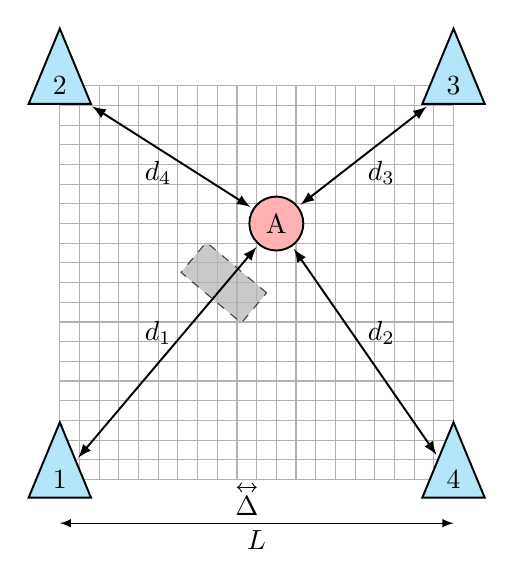
\begin{tikzpicture}
    \newlength{\lato} 
    \setlength{\lato}{5cm}

    \draw[step=\lato/20,black!30,thin] (-\lato/2,-\lato/2) grid (\lato/2,\lato/2);

    \node [isosceles triangle,
    draw,
    fill=cyan!30,
    minimum width =\lato/10,
    minimum height=\lato/20,
    rotate=90,
    line width=0.7pt] (anchor1) at (-\lato/2,-\lato/2) {\rotatebox{-90}{1}};

    \node [isosceles triangle,
    draw,
    fill=cyan!30,
    minimum size =\lato/10,
    rotate=90,
    line width=0.7pt] (anchor2) at (-\lato/2,\lato/2) {\rotatebox{-90}{2}};

    \node [isosceles triangle,
    draw,
    fill=cyan!30,
    minimum size =\lato/10,
    rotate=90,
    line width=0.7pt] (anchor3) at (\lato/2,\lato/2) {\rotatebox{-90}{3}};

    \node [isosceles triangle,
    draw,
    fill=cyan!30,
    minimum size =\lato/10,
    rotate=90,
    line width=0.7pt] (anchor4) at (\lato/2,-\lato/2) {\rotatebox{-90}{4}};

    \node [circle,
    draw,
    fill=red!30,
    minimum size =\lato/30,
    line width=0.7pt] (agent) at (\lato/20*1,\lato/20*3) {A};

    \node [draw, 
    rectangle, 
    dashed,
    minimum width = \lato/5, 
    minimum height = \lato/10,
    rotate=-40,
    fill=black!30,
    opacity=0.7] at (-\lato/12,0) {};
    
    \path [draw, latex-latex, line width=0.7pt, shorten <=1pt, shorten >=1pt] (anchor1) -- (agent){};
    \node at (-\lato/4,-\lato/5+\lato/14) {$d_1$};
    \path [draw, latex-latex, line width=0.7pt, shorten <=1pt, shorten >=1pt] (anchor2) -- (agent) {};
    \node at (\lato/4+\lato/15,-\lato/5+\lato/14) {$d_2$};
    \path [draw, latex-latex, line width=0.7pt, shorten <=1pt, shorten >=1pt] (anchor3) -- (agent) {};
    \node at (\lato/4+\lato/15,\lato/3-\lato/18) {$d_3$};
    \path [draw, latex-latex, line width=0.7pt, shorten <=1pt, shorten >=1pt] (anchor4) -- (agent) {};
    \node at (-\lato/4,\lato/3-\lato/18) {$d_4$};

    \draw [<->, latex-latex] (-\lato/2,-\lato/2-\lato/9) -- (\lato/2,-\lato/2-\lato/9);
    \node at (0,-\lato/2-\lato/6.5) {$L$};

    \draw [<->] (-\lato/20,-\lato/2-\lato/50) -- (0,-\lato/2-\lato/50);
    \node at (-\lato/20+\lato/40,-\lato/2-\lato/15) {$\Delta$};

\end{tikzpicture}

\end{document}